\documentclass[11pt]{article}
\synctex=1

\usepackage[in]{fullpage}
\usepackage{enumitem}

% refs
\usepackage[hidelinks]{hyperref}
\usepackage[square,numbers]{natbib}

% figures and tables
\usepackage{graphicx}
\usepackage{subcaption}

% maths and algorithms
\usepackage{amsmath}
\usepackage{amssymb}
\usepackage{amsthm}
\usepackage{bm}
\usepackage{algorithmic}
\usepackage{algorithm}
\usepackage{mathletters}

\DeclareMathOperator*{\argmax}{argmax}
\DeclareMathOperator*{\argmin}{argmin}
\DeclareMathOperator*{\eqdef}{\stackrel{def}{=}}

\newtheorem{definition}{Definition}
\newtheorem{example}{Example}
\newtheorem{fact}{Fact}
\newtheorem{lemma}{Lemma}
\newtheorem{proposition}{Proposition}
\newtheorem{remark}{Remark}
\newtheorem{theorem}{Theorem}

\usepackage{siunitx}

% used for repeat theorem number with same formatting
\makeatletter
\newenvironment{theorepeat}[1]{\textbf{\@begintheorem{#1}}{\unskip}\itshape}{\@endtheorem}
\makeatother

\setlength{\parindent}{0ex}
\setlength{\parskip}{3pt} 

\begin{document}

% \title{Estimating Quality in User-Guided\\Multi-Objective Bandits Optimization}
\title{Estimating Quality in Multi-Objective Bandits Optimization}

\author{Audrey Durand and Christian Gagn\'e \\
Computer Vision and Systems Laboratory \\
% Department of Electrical Engineering and Computer Engineering \\
Universit\'e Laval, Qu\'ebec (QC), Canada\\
\{ audrey.durand.2@ulaval.ca, christian.gagne@gel.ulaval.ca \}
}

\maketitle

\begin{abstract}
    \begin{abstract}
%Although Deep Convolutional Neural Networks (CNNs) have liberated their power in various computer vision tasks, the most important components of CNN, convolutional layers and fully connected layers, are still limited to linear transformations. In this paper, we propose a novel Factorized Bilinear (FB) layer to model the pairwise feature interactions by considering the quadratic terms in the transformations. Compared with existing methods that tried to incorporate complex non-linearity structures into CNNs, the factorized parameterization makes our FB layer only require a linear increase of parameters and affordable computational cost. To further reduce the risk of overfitting of the FB layer, a specific remedy called DropFactor is devised during the training process. We also analyze the connection between FB layer and some existing models, and show FB layer is a generalization to them. Finally, we validate the effectiveness of FB layer on several widely adopted datasets including CIFAR-10, CIFAR-100 and ImageNet, and demonstrate superior results compared with various state-of-the-art deep models.

Neural Style Transfer~\cite{neuralart} has recently demonstrated very exciting results which catches eyes in both academia and industry. Despite the amazing results, the principle of neural style transfer, especially why the Gram matrices could represent style remains unclear. In this paper, we propose a novel interpretation of neural style transfer by treating it as a domain adaptation problem. Specifically, we theoretically show that matching the Gram matrices of feature maps is equivalent to minimize the Maximum Mean Discrepancy (MMD) with the second order polynomial kernel. Thus, we argue that the essence of neural style transfer is to match the feature distributions between the style images and the generated images. To further support our standpoint, we experiment with several other distribution alignment methods, and achieve appealing results. We believe this novel interpretation connects these two important research fields, and could enlighten future researches.

\end{abstract}
\end{abstract}

\section{Introduction}
Water-in-oil emulsions are commonly formed during petroleum production and pose serious threats to installations and quality of the final product. The electrical phase separation has been used in the petroleum industry for separating water-in-crude oil dispersion's by applying a high electric field onto the flowing emulsion to affect flocculate and coalescence of dispersed water droplets \cite{Cottrell1991,eow02}.
%Cottrell19912, 2001173,  
It has been realized that the emulsion is stabilized by a thin film formed between two drops when approaching each other. Thus demulsification requires rupturing of this thin liquid film. 
%\cite{Bhardwaj1994}. 
Generally, the main purpose of an applied electrical field is to promote contact between the drops and to help in drop\textendash drop coalescence. Pulsed DC (direct current) and AC (alternative current) electric fields are preferred over constant DC fields for efficient coalescence. Recent studies have helped to clarify important aspects of the process such as partial coalescence and drop\textendash drop non-coalescence but key phenomena such as thin film breakup and chain formation are still unclear \cite{Mhatre2015}.
Despite of the tremendous practical importance of enhanced coalescence, the mechanism of separation  is not fully understood \cite{Isaacs01} beyond the  perception that the electrical force facilitates the coalescence between small drops.\\
To help in understanding the inherent processes, computational models were designed  to simulate coalescense of droplets under realistic experimental conditions. Molecular dynamics (MD) method is an useful tool for the purpose.  Koplik and Banavar \cite{Koplik2} did a pioneer work in modeling the coalescence of two Lennard-Jones liquid droplets in a second immiscible fluid using MD simulations. The authors found that coalescence of liquid droplets  was completely driven by van der Waals and electrostatic interactions when the velocities of the droplets were small. The coalescence began when the molecules on the boundary of one droplet thermally drifted to the range of attraction of the other droplet and formed a string to attract both sides of the molecules. \\
Zhao et al.\cite{Zhao2004} reported a MD study of the coalescence of two nanometer-sized water droplets in n-heptane, a system that is commonly encountered in the oil sands industry. Similarly, the coalescence process was initiated by the molecules at the edge of the clusters, which interacted with each other and formed a bridge between two clusters. Eventually, these molecules attracted and pulled out other molecules from their own respective cluster to interact with those from the other cluster. Authors made an important conclusion that the coalescence in n-heptane would occurred only if the two droplets were very close to each other ($\sim 0.5\, nm$). If they were far apart (e.g., $1\, nm$), external driving forces should be applied. 

However, experimental results for electrical properties and electric field-induced rupture of single thin films are scarce, which limits the comparison with computations to several measurable quantities - pore formation, and the critical voltage for film rupture.\\ Anklam et al.  \cite{Anklam1999} experimentally demonstrated that the electric-filed induced pore formation was the reason for break-up of emulsion films. Panchev et al. \cite{Panchev200874} 
developed a method allowing simultaneous investigation of a single water-in-oil emulsion film by both microinterferometry and electrical measurements. This method allows in a single experiment to measure the critical voltage of film rupture, the film thickness, the drainage rate, and the disjoining pressure laying the groundwork for computational studies. \\
 
In this paper we present computational results for pore formation and film rupture obtained with a model, which we have designed to imitate the rupture of the film under a step-wise increase of the electric field as it has been applied  in the experiment \cite{Panchev200874}. The film is immersed in a sodium chloride solution. In the model and also in the experiment, the electric field is applied perpendicularly to the film, which separates two water droplets.\\

The model of the thin film developed for the present study can be considered as a useful starting basis  for a further study of the stability and the structure of thick emulsion films that are stabilized by indigenous crude oil surfactants, namely asphaltenes, resins and naphthenic acids. It is worth mentioning that so far there is almost complete lack of understanding of the intimate structural details of the crude petroleum-like films. Therefore, current industrial practice of utilization of chemical additives in combination with electric field applications has for long time been widely viewed as a ``work of art''. 


%!TEX root = /Users/audrey/Dropbox/PhD/MOMAB/ArXiv/Latex/paper.tex

\section{Multi-Objective Bandits}
\label{sec:momab}

A multi-objective bandits problem is described by a (finite) set of actions $\cA$, also referred to as the \emph{design space}, each of which is associated with a $d$-dimensional expected outcome $\bsmu_a = (\mu_{a, 1}, \dots, \mu_{a, d}) \in \cX \in \Real^d$. For simplicity, we assume that the \emph{objective space} $\cX = [0, 1]^d$. In this episodic game, an agent interacts with an environment characterized by a \emph{preference function}~$f$. The agent iteratively chooses to perform an action $a(t)$ and obtains a noisy observation of $\bsz(t)$.\footnote{Scalars are written unbolded; vectors are boldfaced. The operators $+$, $-$, $\times$, and~$\div$ applied on a vector $\bsv = (v_1, \dots, v_d)$ and a scalar $s$ correspond to the operation between each item of $\bsv$ and $s$, e.g., $\bsv + s = (v_1 + s, \dots, v_d + s)$. These operators applied on two vectors $\bsv = (v_1, \dots, v_d)$ and $\bsu = (u_1, \dots, u_d)$ correspond to itemwise operations between $\bsv$ and $\bsu$, e.g., $\bsv + \bsu = (v_1 + u_1, \dots, v_d + u_d)$.}

An algorithm for a multi-objective bandits problem is a (possibly randomized) method for choosing which action to play next, given a history of previous choices and obtained outcomes, $\cH_t = \{ a(s), \bsz(s) \}_{s = 1}^{t-1}$. Let $\cO = \argmax_{a \in \cA} f(\bsmu_a)$ and let $\star \in \cO$ denote the optimal action. The optimal gap $\Delta_a = f(\bsmu_\star)- f(\bsmu_a)$ measures the expected loss of playing action $a$ instead of the optimal action. The agent's goal is to design an algorithm with low expected (cumulative) regret\footnote{Also known as the scalarized regret~\cite{Drugan2013}.}:
\begin{align}
\label{eqn:regret}
    \kR(T)
    = \sum_{t=1}^T \big( f(\bsmu_\star) - f(\bsmu_{a(t)}) \big)
    = \sum_{t = 1}^T \sum_{a \in \cA} \Pr[a(t) = a] \Delta_a.
\end{align}
This quantity measures the expected performance of the algorithm compared to the expected performance of an optimal algorithm given knowledge of the outcome distributions, i.e., always sampling from the distribution with the expectation maximizing $f$. Typically, we assume that the algorithm maintains one estimate $\bstheta_a(t)$ per action $a$ on time $t$. Let $\cO(t) = \argmax_{a \in \cA} f(\bstheta_a(t))$ denote the set of actions with an estimate maximizing $f$. The algorithm faces a trade-off between playing an action $a(t) \in \cO(t)$ and choosing to gather an additionnal sample from a relatively unexplored action in order to improve its estimate. Alg.~\ref{alg:mobandits} describes this multi-objective bandits problem.

\begin{algorithm}[t]
    On each episode $t \geq 1$:
    \begin{enumerate}[nolistsep]
        \item The agent selects action $a(t)$ to play given $\cO(t)$.
        \item The agent observes $\bsz(t) = \bsmu_{a(t)} + \bsxi(t)$, where $\bsxi(t)$ are i.i.d. random vectors.
        \item The agent updates its estimates.
    \end{enumerate}
    \caption{Multi-objective bandits setting}
\label{alg:mobandits}
\end{algorithm}

In many situations, the environment providing the preference function is a person, let us call her the \emph{expert user}. Unfortunately, people are generally unable to scalarize their choices and preferences. Therefore they cannot explicitely provide their preference function. However, given several options, users can tell which one(s) they prefer (that is $\cO(t)$) and thus can be used as a black box to provide feedback in the learning loop.
% Alg.~\ref{alg:mobandits_user} describes the user-guided multi-objective bandits problem.
%
% \begin{algorithm}[t]
%     On each episode $t \geq 1$:
%     \begin{enumerate}[nolistsep]
%         \item The agent selects action $a(t) \in \cO(t)$ to play.
%         \item The agent observes $\bsz(t) = \bsmu_{a(t)} + \bsxi(t)$, where $\bsxi(t)$ are i.i.d. random variables.
%         \item The agent updates its estimates.
%         \item The agent shows options $\{ \bstheta_a(t) \}_{a \in \cA}$ to the expert user.
%         \item The expert user indicates its preference $\cO(t) = \argmax_{a \in \cA} f(\bstheta_a(t))$.
%     \end{enumerate}
%     \caption{User-guided multi-objective bandits setting}
% \label{alg:mobandits_user}
% \end{algorithm}


\paragraph{Pareto-optimality}

Given two $d$-dimensional options $\bsx = (x_1, \dots, x_d)$ and $\bsy = (y_1, \dots, y_d)$, $\bsx$ is said to dominate, or Pareto-dominate, $\bsy$ (denoted $\bsx \succeq \bsy$) if and only if $x_i > y_i$ for at least one $i$ and $x_i \geq y_i$ otherwise. The dominance is strict (denoted $\bsx \succ \bsy$) if and only if $x_i > y_i$ for all $i = 1, \dots, d$. Finally, the two vectors are incomparable (denoted $\bsx \parallel \bsy$) if $\bsx \nsucc \bsy$ and $\bsy \nsucc \bsx$. Pareto-optimal options represent the best compromises amongst the objectives and are the only options that need to be considered in an application. We say that these options constitute the Pareto front $\cP = \{ a : \nexists \bsmu_b \succeq \bsmu_a \}_{a, b \in \cA}$. Fig.~\ref{fig:pareto_front} shows an example of dominated and non-dominated expected outcomes in a $d = 2$ objectives space. A user facing a multi-criteria decision making problem must select her preferred non-dominated option. Dominated options are obviously discarded by default.

\begin{figure}[t]
    \centering
    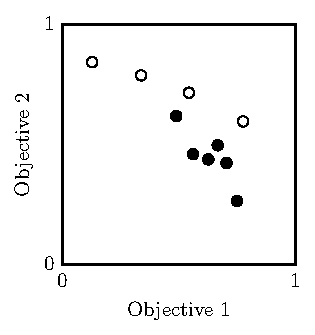
\includegraphics[scale=0.75]{pareto_front}
    \caption{Example of dominated (black) and non-dominated (white) options.}
\label{fig:pareto_front}
\end{figure}


\paragraph{Related Works}

The multi-objective bandits problem has already been addressed in the a posteriori setting, where the goal is to discover the whole Pareto front for a posteriori decision making~\cite{Drugan2013,Yahyaa2015}. This is different from the a priori optimization problem tackled here. The aim of algorithms in the a posteriori setting is to simultaneously minimize the Pareto-regret and the unfairness metrics. Also known as the $\epsilon$-distance~\cite{Laumanns2002}, the Pareto-regret associated with playing action $a$ is the minimum value $\epsilon_a$ such that $\bsmu_a + \epsilon_a$ is not dominated by any other actions. In other words, any action standing on the front is considered equally good by the expert user. This is like considering that $\cO = \cP$, which corresponds to the preference function $f(\bsmu_\star) = 1$, $f(\bsmu_a) = 1 - \epsilon_a$, such that $\Delta_a = \epsilon_a$. Note that any algorithm optimizing a single objective could minimize the Pareto-regret regardless of the other objectives. This is addressed by the unfairness metric, measuring the disparity in the amount of plays of non-dominated actions -- the idea being to force algorithms to explore the whole Pareto front evenly.

In MOO settings~\cite{Zuluaga2013}, the goal is to identify the Pareto-optimal set $\cP$ without evaluating all actions. The quality of a solution $\cS$ is typically given by the hypervolume error $V(\cP) - V(\cS)$, where the $V(\cP)$ is the volume enclosed between the origin and $\{ \bsmu_a \}_{a \in \cP}$ (and similarly for $\cS$). However, the hypervolume error does not give information about the quality of the estimation of actions. Identifying the Pareto front alone does not guarantee that the actions are well estimated and, therefore, that an expert user choice based on these estimations would lead to the right choice.


%!TEX root = /Users/audrey/Dropbox/PhD/MOMAB/ArXiv/Latex/paper.tex

\section{Preference Radius}
\label{sec:preference_radius}

Let $\bstheta_a(t)$ denote the estimation associated with action $a$ on episode $t$ and let $\cP(t) = \{ a : \nexists \bstheta_b(t) \succ \bstheta_a(t) \}_{a, b \in \cA}$ denote the estimated Pareto front given these options. By definition, the optimal options are $\cO(t) \subseteq \cP(t)$. Let
\begin{align*}
    B(\bsc, r) \subseteq \{ \bsx \in \cX : |x_i - c_i| < r, ~ i = 1, \dots, d \}
\end{align*}
denote a ball of center $\bsc$ and radius $r$. In order to characterize the difficulty of a multi-objective bandits setting, we introduce the following quantity.
%
\begin{definition}
For each action $a \in \cA$, we define the preference radius $\rho_a$ as any radius such that if $\bstheta_a(t) \in B(\bsmu_a, \rho_a)$ for all actions, then
\begin{align*}
    \exists \star \in \cO : \star \in \cO(t) \quad \text{and} \quad a \not\in \cO(t) ~ \forall a \in \cA, a \not\in \cO.
\end{align*}
\end{definition}
%
The radii correspond to the \emph{robustness} of the preference function, that is to which extent can actions be poorly estimated simultaneously before the set of optimal options changes. The radius $\rho_a$ is directly linked to the gap $\Delta_a = f(\bsmu_\star)- f(\bsmu_a)$. For a suboptimal action, a large radius indicates that this action is far from being optimal. Also, the preference radii of suboptimal actions depend on the preference radius of the optimal action(s). Larger optimal action radii imply smaller radii for suboptimal actions. Note that if all actions estimates stand in their preference balls, being greedy is optimal.

Let $\alpha_1, \dots, \alpha_d \in [0, 1]$ denote \emph{weights} such that $\sum_{i = 1}^d \alpha_i = 1$. The weighted $L_p$ metric $f(\bsx)= \big( \sum_{i = 1}^d \alpha_i x_i^p \big)^{1/p}$ with $p \geq 1$ is often used to represent decision functions. This function is known as the linear scalarization when $p = 1$ and as the Chebyshev scalarization when $p = \infty$. The following examples show the link between the preference radii and the gap for these two common functions.

\begin{figure}[t]
    \centering
    \begin{subfigure}[b]{0.35\textwidth}
        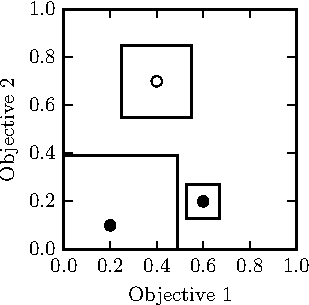
\includegraphics[scale=0.75]{pref_radius_weighted_sum_2}
    \end{subfigure}
    \qquad
    \begin{subfigure}[b]{0.35\textwidth}
        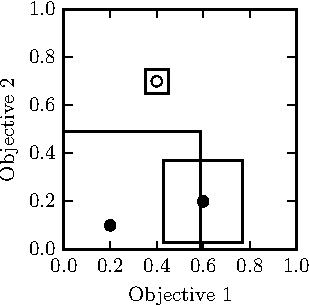
\includegraphics[scale=0.75]{pref_radius_weighted_sum_1}
    \end{subfigure}
    \caption{Examples of preference radii around the optimal (white) and suboptimal (black) actions given the linear preference function $f(\bsx) = 0.4 x_1 + 0.6 x_2$.}
\label{fig:pref_radius:example:weigthed_sum}
\end{figure}

\begin{example}[Linear]
\label{ex:linear}
    The linear scalarization function is given by
    \begin{align*}
        f(\bsx) = \sum_{i = 1}^d \alpha_i x_i.
    \end{align*}
    Consider the optimal action $\star$ and the suboptimal action $a$. By definition of the preference radii, we have that
    \begin{align*}
        \min_{\bstheta_\star \in B(\bsmu_\star, \rho_\star)} f(\bstheta_\star) & > \max_{\bstheta_a \in B(\bsmu_a, \rho_a)} f(\bstheta_a) \\
        \sum_{i = 1}^d (\alpha_i \mu_{\star, i} - \alpha_i \rho_\star) &> \sum_{i = 1}^d (\alpha_i \mu_{a, i} + \alpha_i \rho_a) \\
        f(\bsmu_\star) - \rho_\star & > f(\bsmu_a) + \rho_a \\
        \Delta_a & > \rho_\star + \rho_a.
    \end{align*}
    Fig.~\ref{fig:pref_radius:example:weigthed_sum} shows examples of preference radii with a linear preference function.
%In both cases, as long as each option stays in its associated radius, the expert user preference won't change.
\end{example}

\begin{example}[Chebyshev]
\label{ex:chebyshev}
    The Chebyshev scalarization~\cite{Bowman1976} function is given by
    \begin{align*}
        f(\bsx) = \max_{1 \leq i \leq d} \alpha_i x_i.
    \end{align*}
    Consider the optimal and suboptimal actions $\star$ and $a$, and let
    \begin{align*}
        i_\star = \argmax_{1 \leq i \leq d} \alpha_i (\mu_{\star, i} - \rho_\star), \quad
        i_a = \argmax_{1 \leq i \leq d} \alpha_i (\mu_{a, i} - \rho_a).
    \end{align*}
    By definition of the preference radii, we have that
    \begin{align*}
        \min_{\bstheta_\star \in B(\bsmu_\star, \rho_\star)} f(\bstheta_\star) & > \max_{\bstheta_a \in B(\bsmu_a, \rho_a)} f(\bstheta_a) \\
        \max_{1 \leq i \leq d} \alpha_i (\mu_{\star, i} + \rho_\star) & > \max_{1\leq i \leq d} \alpha_i (\mu_{a, i} - \rho_a) \\
        \alpha_{i_\star} \mu_{\star, i} - \alpha_{i_\star} \rho_\star & > \alpha_{i_a} \mu_{a, i} + \alpha_{i_a} \rho_a  \\
        f(\bsmu_\star) - \alpha_{i_\star} \rho_\star &> f(\bsmu_a) + \alpha_{i_a} \rho_a \\
        \Delta_a &> \alpha_{i_\star} \rho_\star + \alpha_{i_a} \rho_a.
    \end{align*}
    The difficulty here is that $i_\star$ and $i_a$ respectively depend on $\rho_\star$ and $\rho_a$. Consider a 2-objective setting, we can define
    \begin{align*}
        \tau_\star = \frac{\alpha_2 \mu_{\star, 2} - \alpha_1 \mu_{\star, 1}}{\alpha_2 - \alpha_1}, \quad
        \tau_a = \frac{\alpha_1 \mu_{a, 1} - \alpha_2 \mu_{a, 2}}{\alpha_2 - \alpha_1}
    \end{align*}
    as thresholds such that
    \begin{align*}
        i_\star = \bigg\{
            \begin{array}{ll}
            1 & \quad \text{if} \quad \rho_\star > \tau_\star \\
            2 & \quad \text{otherwise}
            \end{array}, \quad
        i_a = \bigg\{
            \begin{array}{ll}
            1 & \quad \text{if} \quad \rho_a < \tau_a \\
            2 & \quad \text{otherwise}.
            \end{array}
    \end{align*}
    %
    Fig.~\ref{fig:pref_radius:example:chebyshev} shows examples of preference radii with a Chebyshev preference function. 
\end{example}

\begin{figure}[t]
    \centering
    \begin{subfigure}[b]{0.35\textwidth}
        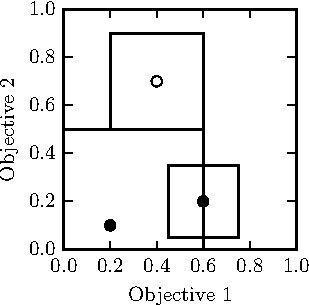
\includegraphics[scale=0.75]{pref_radius_chebyshev_2}
    \end{subfigure}
    \qquad
    \begin{subfigure}[b]{0.35\textwidth}
        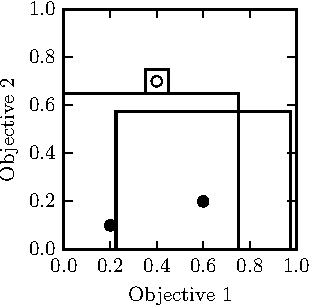
\includegraphics[scale=0.75]{pref_radius_chebyshev_1}
    \end{subfigure}
    \caption{Examples of preference radii around the optimal action (white) and suboptimal actions (black) given a Chebyshev function with $\alpha_1 = 0.4$ and $\alpha_2 = 0.6$.}
\label{fig:pref_radius:example:chebyshev}
\end{figure}

Outside $L_p$ metrics, other scalarization functions are often based on constraints. For example, using the $\epsilon$-constraint scalarization technique, a user assigns a constraint to every objective except a target objective $\ell$. All options that fail to respect one of the contraints receive a value of 0, while the options that respect all constraints get a value of $x_\ell$. The following example shows the relation between the preference radius and the gap given a preference function that is articulated as an $\epsilon$-constraint scalarization technique.
%
\begin{example}[Epsilon-constraint]
\label{ex:epsilon-constraint}
    The $\epsilon$-constraint function is given by
    \begin{align*}
    f(\bsx) = \bigg\{
        \begin{array}{ll}
        x_\ell & \quad \text{if} \quad x_i \geq \epsilon_i \quad \forall i \in \{ 1, \dots, d \}, i \neq \ell \\
        0 & \quad \text{otherwise}.
        \end{array}
    \end{align*}
    Consider the optimal and suboptimal actions $\star$ and $a$. By definition of the preference radii, we have that
    \begin{align*}
        \rho_\star \leq \min_{1 \leq i \leq d, i \neq \ell} \mu_{\star, i} - \epsilon_i.
    \end{align*}
    We decompose $\rho_a = \ubar{\rho}_a + \bar{\rho}_a$ such that
    \begin{align*}
        \ubar{\rho}_a = \min \{ 0, \max_{1 \leq i \leq d, i \neq \ell} \epsilon_i - \mu_{a, i} \}
    \end{align*}
    denotes the radius required in order for action a to respect the constraints, that is to obtain $f(\bsmu_a) > 0$, and $\bar{\rho}_a$ denotes the leftover leading to a gap reduction. Finally, we have that
    \begin{align*}
        \mu_{\star, \ell} - \rho_\star > \mu_{a, \ell} + \ubar{\rho}_a + \bar{\rho_a} \quad \text{and} \quad
        \Delta_a > \rho_\star + \rho_a.
    \end{align*}
    Fig.~\ref{fig:pref_radius:example:econstraint} shows examples of preference radii with $\epsilon$-constraint preference functions.
\end{example}

\begin{figure}[t]
    \centering
    \begin{subfigure}[b]{0.35\textwidth}
        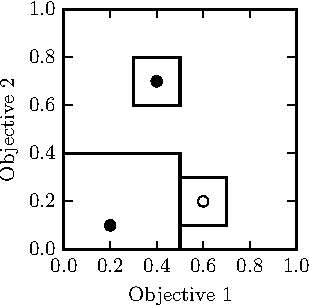
\includegraphics[scale=0.75]{pref_radius_econstraint_f2}
        \caption{$\ell = 1$, $\epsilon_2 = 0.1$}
    \end{subfigure}
    \qquad
    \begin{subfigure}[b]{0.35\textwidth}
        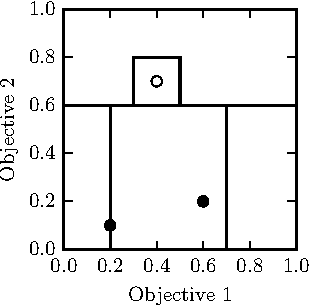
\includegraphics[scale=0.75]{pref_radius_econstraint_f1}
        \caption{$\ell = 2$, $\epsilon_1 = 0.3$}
    \end{subfigure}
    \caption{Examples of preference radii around the optimal (white) and suboptimal (black) actions given two different configurations of $\epsilon$-contraint.}
\label{fig:pref_radius:example:econstraint}
\end{figure}


%!TEX root = /Users/audrey/Dropbox/PhD/MOMAB/ArXiv/Latex/paper.tex

\section{Thompson Sampling}
\label{sec:ts}

% In this section we use the preference radius to analyze the Thompson sampling (TS)~\cite{Thompson1933} algorithm using multivariate normal (MVN) priors. Recall that TS
The Thompson sampling (TS)~\cite{Thompson1933} algorithm maintains a posterior distribution $\pi_a(t)$ on the mean $\bsmu_a$ given a prior and the history of observations $\cH_t$. On each episode $t$, one option $\bstheta_a(t)$ is sampled from each posterior distribution $\pi_a(t)$. The algorithm selects $a(t) \in \cO(t)$. Recall that $\cO(t) = \argmax_{a \in \cA} f(\bstheta_a(t))$. Therefore $\Pr[a(t) = a]$ is proportionnal to the posterior probability that $a$ maximizes the preference function given the history $\cH_t$. Let $N_a(t) = \sum_{s = 1}^{t-1} \ind[a(s) = a]$ denote the number of times action $a$ has been played up to episode $t$. Also let
\begin{align*}
    \hat \bsmu_{a, t} = \frac{\sum_{s = 1: a(s) = a}^{t-1} \bsz(s)}{N_a(t)}
    ~\text{and}~
    \hat \bsSigma_{a, t} = \frac{\sum_{s = 1: a(s) = a}^{t - 1} \big( \bsz(s) - \hat \bsmu_a(t) \big) \big( \bsz(s) - \hat \bsmu_a(t) \big)^\top}{N_a(t) - 1}
\end{align*}
respectively denote the empirical mean and covariance, and let $\bsSigma_0$ and $\bsmu_0$ denote priors. For MVN priors, the posterior over $\bsmu_a$ is given by a MVN distribution $\Normal_d (\tilde \bsmu_a(t), \tilde \bsSigma_a(t))$, where
\begin{align*}
    \tilde \bsSigma_a(t) = \big( \bsSigma_0^{-1} + N_a(t) \bsSigma_a^{-1} \big)^{-1} ~ \text{and} ~
    \tilde \bsmu_a(t) = \tilde \bsSigma_a(t) \big( \bsSigma_0^{-1} \bsmu_0 + N_a(t) \bsSigma_a^{-1} \hat \bsmu_a(t) \big)
\end{align*}
for the known covariance matrix $\bsSigma_a$. Since assuming that $\bsSigma_a$ is known might be unrealistic in practice, one can consider the non-informative covariance $\bsSigma_a = \bsI_d$. With non-informative priors $\bsmu_0 = \bszero_{d \times 1}$ and $\bsSigma_0 = \bsI_d$,\footnote{$\bszero_{d \times 1}$ indicates a $d$-elements column vector and $\bsI_d$ indicates a $d \times d$ identity matrix.} this corresponds to a direct extension of the one-dimensional TS from Gaussian priors~\cite{Agrawal2013}. Alg.~\ref{alg:mvn_ts} shows the resulting TS procedure from MVN priors.

\begin{algorithm}[t]
    \begin{algorithmic}[1]
        \FORALL{episode $t \geq 1$}
            \FORALL{action $a \in \cA$}
                \STATE sample $\bstheta_a(t) = \Normal_d \big( (\bsI_d + N_a(t) \bsI_d)^{-1} N_a(T) \hat \bsmu_a(t), (\bsI_d + N_a(t) \bsI_d)^{-1} \big)$
            \ENDFOR
            \STATE $\cO(t) = \argmax_{a \in \cA} f(\bstheta_a(t))$
            \STATE play $a(t) \in \cO(t)$ and observe $\bsz(t)$
        \ENDFOR
    \end{algorithmic}
    \caption{Thompson sampling from MVN priors}
\label{alg:mvn_ts}
\end{algorithm}

The following proposition provides general regret bounds for TS from MVN priors. The next theorem specializes these regret bounds for three well known preference function families using the relation between preference radii and the gap, as discussed in previous examples.

\begin{proposition}
\label{prop:mvn_ts}
    Assuming $\sigma$-sub-Gaussian noise with $\sigma^2 \leq 1/(4d)$, the expected regret of TS from MVN priors (Alg.~\ref{alg:mvn_ts}) is bounded by
    \begin{align*}
        \kR(T)
        & \leq \sum_{a \in \cA, a \neq \star} \bigg[
        (C(d) + 4d) (1 + \sigma) \Delta_a \frac{\ln(d T \Delta_a^2)}{\rho_\star^2} + \frac{4}{\Delta_a}
        + 2 \Delta_a \frac{\ln(d T \Delta_a^2)}{(\rho_a - r_a)^2} \\
        & \qquad \qquad \quad + 2 \sigma^2 \Delta_a \frac{\ln(d T \Delta_a^2)}{r_a^2} \bigg],
    \end{align*}
    where $\rho_\star$, $\rho_a$ are preference radii, $r_a < \rho_a$, and $C(d)$ is such that $e^{-\frac{\sqrt{i}}{\sqrt{18 \pi d \ln i}^d}}\leq \frac{d}{i^2}$ for $i \geq C(d)$ (see Remark~\ref{remark:const_c}).
\end{proposition}

\begin{theorem}
\label{thm:mvn_ts}
    Assume either a linear (Ex.~\ref{ex:linear}), Chebyshev (Ex.~\ref{ex:chebyshev}), or $\epsilon$-constraint (Ex.~\ref{ex:epsilon-constraint}) preference function. Assuming $\sigma$-sub-Gaussian noise with $\sigma^2 \leq 1/(4d)$, the expected regret of TS from MVN priors (Alg.~\ref{alg:mvn_ts}) is bounded by
    \begin{align*}
        \kR(T) \leq \sum_{a \in \cA, a \neq \star} \bigg[
        (8C(d) + 24d + 18 + 72\sigma^2) (1 + \sigma)^2 \frac{\ln(d T \Delta_a^2)}{\Delta_a} + \frac{4}{\Delta_a} \bigg],
    \end{align*}
    where $C(d)$ is such that $e^{-\frac{\sqrt{i}}{\sqrt{18 \pi d \ln i}^d}} \leq \frac{d}{i^2}$ for $i \geq C(d)$ (see Remark~\ref{remark:const_c}). This regret bound is of order $\cO(\sqrt{dNT}\ln d + \sqrt{dNT \ln N})$, where $N = |\cA|$. More specifically, for $d \leq \ln N$, it is of order $\cO(\sqrt{dNT \ln N})$.
\end{theorem}

\begin{remark}
\label{remark:const_c}
    For $d = 1$ we can take $C(d) = e^{14}$. For $d = 2$ we can take $C(d) = e^{24}$, for $d = 3$ we can take $C(d) = e^{35}$, and so on for any $d \in \Nat$.
\end{remark}

For $d = 1$, the order of the regret bounds given by Theorem~\ref{thm:mvn_ts} match the order of the regret bounds for TS from Gaussian priors in the single-objective bandits setting~\cite{Agrawal2013}, assuming $[0, 1]$-bounded outcomes. However we observe that the noise tolerance decreases linearly with the dimension $d$ of the objective space. This means that the more dimensions we have, the less noise we can bear in order for these bounds to hold, \emph{given the provided analysis}. 


%!TEX root = /Users/audrey/Dropbox/PhD/MOMAB/ArXiv/Latex/paper.tex

\section{Theoretical Analysis}
\label{sec:analysis}

In this section we start by proving Prop.~\ref{prop:mvn_ts} that provides a regret bound for TS with MVN priors that is independent from the preference function. Then we use the relations between the gap and the preference radius in three preference function families to obtain Theorem~\ref{thm:mvn_ts}.

\subsection{Proof of Prop.~\ref{prop:mvn_ts}}

The following analysis extends the work for the 1-dimensional setting~\cite{Agrawal2013} to the $d$-dimensional setting. We rewrite Eq.~\ref{eqn:regret} as
\begin{align*}
    \kR(T) = \sum_{a \in \cA, a \neq \star} \Delta_a \sum_{t = 1}^T \Pr[a(t) = a],
\end{align*}
where we control $\sum_{t = 1}^T \Pr[a(t) = a]$. The proof relies on several facts (see Appendix~\ref{app:technical_tools}) that extend Chernoff's inequalities and (anti-)concentration bounds from the $1$-dimensional setting to the $d$-dimensional setting using the concepts of Pareto-domination and preference radius. We introduce the following quantities and events to control the quality of mean estimations and the quality of samples.

\begin{definition}[Quantities $r_a$]
    For each suboptimal action $a$, we choose a quantity $r_a < \rho_a$, where $\rho_a$ is a preference radius. By definition of the preference radii, we have $\bsmu_a \prec \bsmu_a + r_a \prec \bsmu_a + \rho_a$. Recall that $f(\bsx) < f(\bsy)$ if $\bsx \prec \bsy$. Hence we have $f(\bsmu_a) < f(\bsmu_a + r_a) < f(\bsmu_a + \rho_a) < f(\bsmu_\star - \rho_\star)$.
\end{definition}

\begin{definition}[Events $E_a^\mu(t)$, $E_a^\theta(t)$]
    For each suboptimal action $a$, define $E_a^\mu(t)$ as the event that $\hat \bsmu_a(t) \prec \bsmu_a + r_a$, and define $E_a^\theta(t)$ as the event that $\bstheta_a(t) \prec \bsmu_a + \rho_a$. More specifically, they are the event that suboptimal action $a$ is well estimated and well sampled, respectively.
\end{definition}

\begin{definition}[Filtration $\cF_t$]
    Define filtration $\cF_t = \{ a(s), \bsz(s) \}_{s = 1, \dots, t-1 }$.
\end{definition}

For suboptimal action $a$, we decompose
\begin{align*}
    \sum_{t=1}^T \Pr[a(t) = a]
    % & = \sum_{t=1}^T \Pr[a(t) = a] \\
    & = \underbrace{\sum_{t=1}^T \Pr[a(t) = a, E_a^\mu(t), E_a^\theta(t)]}_{\text(A)}
    + \underbrace{\sum_{t=1}^T \Pr[a(t) = a, E_a^\mu(t), \overline{E_a^\theta(t)}]}_{\text(B)}
    + \underbrace{\sum_{t=1}^T \Pr[a(t) = a, \overline{E_a^\mu(t)}]}_{\text(C)}
\end{align*}
and control each part separately. In (A), $a$ is played while being well estimated and well sampled. We control this by bounding poor estimation and poor samples for the optimal action. In (B), $a$ is played while being well estimated but poorly sampled. We control this using Gaussian concentration inequalities. In (C), $a$ is played while being poorly estimated. We control this using Chernoff inequalities. Gathering the following results together
% , we obtain
% \begin{align*}
%     \Delta_a \Esp[N_a(T)]
%     & \leq \Delta_a (2C(d) + 8d) (1 + \sigma)^2 \frac{\ln(d T \Delta_a^2)}{\rho_\star^2} + \frac{4}{\Delta_a}
%     + \Delta_a 2 \frac{\ln(d T \Delta_a^2)}{(\rho_a - r_a)^2} \\
%     & \quad + \Delta_a 2 \sigma^2 \frac{\ln(d T \Delta_a^2)}{r_a^2}
% \end{align*}
% for $\sigma^2 \leq 1/(4d)$, where $C(d)$ is such that $e^{-\frac{\sqrt{i}}{\sqrt{18 \pi d \ln i}^d}} \leq \frac{d}{i^2}$ for $i \geq C(d)$.
and summing over all suboptimal actions, we obtain Prop.~\ref{prop:mvn_ts}.


\subsubsection{Bounding (A)}

By definition of TS, for suboptimal $a$ to be played on episode $t$, we must (at least) have $f(\bstheta_a(t)) \geq f(\bstheta_\star(t))$. By definition of event $E_a^\theta(t)$ and the preference radii, we have $f(\bstheta_a(t)) < f(\bstheta_\star(t))$ if $\bstheta_\star(t) \succ \bsmu_\star - \rho_\star$. Let $\tau_k$ denote the time step at which action $\star$ is selected for the $k^\mathrm{th}$ time for $k \geq 1$, and let $\tau_0 = 0$. Note that for any action $a$, $\tau_k > T$ for $k > N_a(T)$ and $\tau_T \geq T$. Then

\begin{align}
\label{eqn:a}
    (A)
    & = \sum_{t=1}^T \Pr[a(t) = a, E_a^\mu(t), E_a^\theta(t) | \cF_t] \nonumber \\
    & \leq \sum_{t=1}^T \Pr[f(\bstheta_a(t)) > f(\bstheta_\star(t)), E_a^\mu(t), E_a^\theta(t) | \cF_t] \nonumber \\
    & \leq \sum_{t=1}^T \Pr[\bstheta_\star(t) \not\succ \bsmu_\star - \rho_\star | \cF_t] \nonumber \\
    & \leq \sum_{k=0}^{L} \Esp \bigg[ \sum_{t=\tau_k+1}^{\tau_{k+1}} \ind[\bstheta_\star \not\succ \bsmu_\star - \rho_\star | \cF_t] \bigg]
    + \sum_{t=\tau_L+1}^T \Pr[\bstheta_\star(t) \not\succ \bsmu_\star - \rho_\star, N_\star(t) > L | \cF_t].
\end{align}
The second inequality uses the fact that the sampling of $\bstheta_\star(t)$ is independent from the events $E_a^\mu(t)$ and $E_a^\theta(t)$. The last inequality uses the observation that $\Pr[\bstheta_\star(t) \not\succ \bsmu_\star - \rho_\star | \cF_t]$ is fixed given $\cF_t$ and that it changes only when $\pi_\star(t)$ changes, that is only when action $\star$ is played. The first sum counts the number of episodes required before action $\star$ has been played $L$ times. The second counts the number of episodes where $\star$ is badly sampled after having been played $L$ times. We use the following Lemma to control the first summation, see Appendix~\ref{app:proof:counts_before_succ}.

\begin{lemma}[Based on Lemma~6 from \cite{Agrawal2013}]
\label{lem:counts_before_succ}
    Let $\tau_k$ denote the time of the $k^\mathrm{th}$ selection of action $\star$. Then, for any $d \in \Nat$ and $\sigma^2 \leq 1/(4d)$,
    \begin{align*}
        \Esp \bigg[ \sum_{t=\tau_k+1}^{\tau_{k+1}} \Pr[\bstheta_\star(t) \not\succ \bsmu_\star - \rho_\star | \cF_t] \bigg]
        \leq C(d) + 4d,
    \end{align*}
    where $C(d)$ is such that $e^{-\frac{\sqrt{i}}{\sqrt{18 \pi d \ln i}^d}} \leq \frac{d}{i^2}$ for $i \geq C(d)$.
\end{lemma}

Now we bound the second summation in Eq.~\ref{eqn:a} by controlling the probability of poorly sampling $\bstheta_\star(t)$ when $N_\star(t) > L$. Let $E_\star(t)$ denote the event that $\hat \bsmu_\star(t) \succ \bsmu_\star - \sigma \rho_\star / (1 + \sigma)$. Then we have
\begin{align*}
    \Pr[\bstheta_\star(t) \not\succ \bsmu_\star - \rho_\star, N_\star(t) > L | \cF_t]
    & \leq \Pr \Big[ \bstheta_\star(t) \not\succ \hat \bsmu_\star(t) - \frac{\rho_\star}{1 + \sigma}, E_\star(t), N_\star(t) > L | \cF_t \Big] \\
    & \qquad + \Pr[\overline{E_\star(t)}, N_\star(t) > L | \cF_t] \\
    & \leq \Pr \Big[ \bstheta_\star(t) \not\in B \Big( \hat \bsmu_\star(t), \frac{\rho_\star}{1 + \sigma} \Big), E_\star(t), N_\star(t) > L | \cF_t \Big] \\
    & \qquad + \Pr \Big[ \hat \bsmu_\star(t) \not\in B \Big( \bsmu_\star - \frac{\sigma \rho_\star}{1 + \sigma} \Big), N_\star(t) > L | \cF_t \Big] \\
    & \leq \frac{d}{2} e^{-\frac{L \rho_\star^2}{2(1 + \sigma)^2}} + 2 d e^{-\frac{L \rho_\star^2}{2(1 + \sigma)^2}}.
\end{align*}
The last inequality uses Facts~\ref{fac:chernoffd} and~\ref{fac:concentration}. With $L = 2 (1 + \sigma)^2 \frac{\ln(d T \Delta_a^2)}{\rho_\star^2}$ we obtain
\begin{align}
\label{eqn:a:prob_bad_theta_star}
    \Pr[\bstheta_\star(t) \not\succ \bsmu_\star - \rho_\star, N_\star(t) > L | \cF_t]
    \leq \frac{5}{2 T \Delta_a^2}.
\end{align}
We use Lem.~\ref{lem:counts_before_succ} and Eq.~\ref{eqn:a:prob_bad_theta_star} in Eq.~\ref{eqn:a} to obtain
\begin{align*}
    (A) \leq (2C(d) + 8d) (1 + \sigma)^2 \frac{\ln(d T \Delta_a^2)}{\rho_\star^2} + \frac{5}{2 \Delta_a^2}
\end{align*}
for $\sigma^2 \leq 1/(4d)$, where $C(d)$ is such that $e^{-\frac{\sqrt{i}}{\sqrt{18 \pi d \ln i}^d}} \leq \frac{d}{i^2}$ for $i \geq C(d)$.


\subsubsection{Bounding (B)}

We control the probability of badly sampling suboptimal action $a$ given that it has been played at least $L$ times. Recall that filtration $\cF_t$ is such that $E_a^\mu(t)$ holds. To that extent we decompose
\begin{align*}
    (B)
    & = \sum_{t=1}^T \Pr[a(t) = a, \overline{E_a^\theta(t)}, E_a^\mu(t), N_a(t) \leq L | \cF_t]
    + \sum_{t=1}^T \Pr[a(t) = a, \overline{E_a^\theta(t)}, E_a^\mu(t), N_a(t) > L | \cF_t] \\
    & \leq \Esp \bigg[ \sum_{t=1}^T \ind[a(t) = a, N_a(t) \leq L | \cF_t] \bigg]
    + \sum_{t=1}^T \Pr[\bstheta_a(t) \not\prec \bsmu_a + \rho_a, N_a(t) > L | \cF_t] \\
    & \leq L + \sum_{t=1}^T \Pr[\bstheta_a(t) \not\prec \hat \bsmu_a(t) + (\rho_a - r_a), N_a(t) > L | \cF_t] \\
    & \leq L + T \frac{d}{2} e^{-\frac{L(\rho_a - r_a)^2}{2}}.
\end{align*}
The first inequality uses the observation that $\Pr[a(t) = a | \cF_t]$ is fixed given $\cF_t$ and the definition of event $\overline{E_a^\theta(t)}$. The second inequality uses the fact that event $E_a^\mu(t)$ holds. The last inequality uses Fact~\ref{fac:concentration}.
% with $\sigma^2 = \frac{1}{N_a(t)+1} \leq \frac{1}{L}$.
With $L = 2 \frac{\ln(d T \Delta_a^2)}{(\rho_a - r_a)^2}$ we obtain
\begin{align*}
    (B) \leq 2 \frac{\ln(d T \Delta_a^2)}{(\rho_a - r_a)^2} + \frac{1}{2 \Delta_a^2}.
\end{align*}


\subsubsection{Bounding (C)}

Similarly to what has been done previously with (B), we can control the probability of badly estimating suboptimal action $a$ given that it has been played at least $L$ times. Then we have
\begin{align*}
    (C)
    & \leq \sum_{t=1}^{T} \Pr[a(t) = a, \overline{E_a^\mu(T)}, N_a(t) \leq L | \cF_t]
    + \sum_{t=1}^T \Pr[a(t) = a, \overline{E_a^\mu(T)}, N_a(T) > L | \cF_t] \\
    & \leq \Esp \bigg[ \sum_{t=1}^T \ind[a(t) = a, N_a(t) \leq L] \bigg] + \sum_{t=1}^T \Pr[\overline{E_a^\mu(T)}, N_a(T) \geq L] \\
    & \leq L + T d e^{-\frac{L r_a^2}{2\sigma^2}}.
\end{align*}
The second inequality uses the observation that $\Pr[a(t) = a | \cF_t]$ is fixed given $\cF_t$. The last inequality uses Fact~\ref{fac:chernoffd}. With $L = 2 \sigma^2 \frac{\ln(d T \Delta_a^2)}{r_a^2}$ we obtain
\begin{align*}
    (C) \leq 2 \sigma^2 \frac{\ln(d T \Delta_a^2)}{r_a^2} + \frac{1}{\Delta_a^2}.
\end{align*}


\subsection{Proof of Theorem~\ref{thm:mvn_ts}}

By definition of the preference radii, given a linear (Ex.~\ref{ex:linear}), Chebyshev (Ex.~\ref{ex:chebyshev}), or $\epsilon$-constraint preference function (Ex.~\ref{ex:epsilon-constraint}), one can take $\rho_\star = \rho_a = \frac{\Delta_a}{2}$, $r_a = \frac{\Delta_a}{6}$. Using these values in Prop.~\ref{prop:mvn_ts}, we obtain Theorem~\ref{thm:mvn_ts}:
\begin{align*}
    \kR(T)
    & \leq \sum_{a \in \cA, a \neq \star} \bigg[
    (8C(d) + 24d + 18 + 72\sigma^2) (1 + \sigma)^2 \frac{\ln(d T \Delta_a^2)}{\Delta_a} + \frac{4}{\Delta_a} \bigg].
\end{align*}
Let $\Delta_a = \delta_a \sqrt{\frac{dN \ln N}{T}}$, for $\delta_a \in (0, \sqrt{\frac{T}{d N \ln N}}]$. The regret is bounded by
\begin{align*}
    \kR(T)
    & \leq (8C(d) + 24d + 18 + 72 \sigma^2) (1 + \sigma)^2  \frac{\sqrt{N T} \ln(d^2 N \ln N)}{\delta_a \sqrt{d \ln N}} + \frac{4 \sqrt{N T}}{\delta_a \sqrt{d \ln N}}
\end{align*}
with $\sigma^2 \leq 1/(4d)$, that is of order $\cO(\sqrt{dNT}\ln d + \sqrt{dNT \ln N})$. More specifically, for $d \leq \ln N$, the regret bound is of order $\cO(\sqrt{dNT \ln N})$.


% !TEX root = ../EDBT.tex
\begin{figure}
\centering
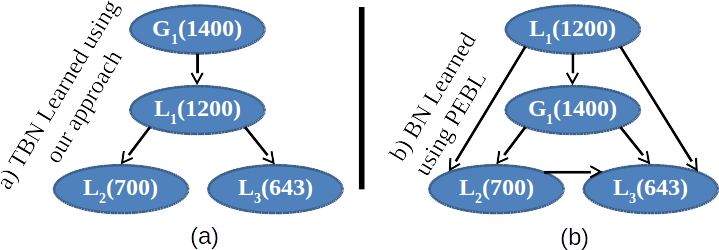
\includegraphics[width = 100mm]{Figures/g1Network.png}
\vspace{6pt}
\caption{Structure learned of $G_1$ using two different approaches}
\label{fig:g1net}
%\vspace{-10pt}
\end{figure}

We present the accuracy of our predictions on a real-life dataset from a global market research organization. We set a threshold $\tau$ on CoP, and predictions with a CoP $< \tau$ are routed for human annotation. We also measure the accuracies of our predictions for different values of $\tau$.

\textit{\textbf{Data description}}: We have data for carbonated drinks of $26$K unique products from a single geography, contained in two datasets:
a)~\textbf{Local DB}: It contains 26K products with each product having $49$ local characteristics, where cardinality of local characteristics varies from tens to thousands. It also contains descriptions of products given by retailers of that product, where number of descriptions of a single product varies from tens to hundreds. b)~\textbf{Global DB}: It contains four global characteristics with cardinality varying from tens to thousands.

\textbf{\textit{Data Preparation:}} We predict four global characteristics $G_1$, $G_2$, $G_3$, and $G_4$ for two cases, with varying ratio of split between training, validation and test datasets. \textbf{\textit{Case-1}}(60:20:20) has 60\% training, 20\% validation and 20\% test and \textbf{\textit{Case-2}} has this ratio as 20:20:60. \textbf{NOTE:} While Case-1 uses a traditional split of training vs testing data, Case-2 is more realistic, since in practice preparing a training data by manual data labeling is costly: For example, we would like to `onboard' a data from a particular dataset 
by manually annotating only a small fraction (e.g. 20\%) of records and automate the remainder or we might like to board 
data from one organization (e.g. retailer or distributor) in a particular geography in the hope that data from remaining sources in that
geography share similar local characteristics, eliminating manual annotation for a large volume of data. 
To simulate this practical scenario, we used the first few records from the local dataset, which happened to contain only 10\% or so of the
total possible values of each global attribute.

For SBM, $\eta$ relevant local characteristics was chosen for every $G_j$. Figure~\ref{fig:g1net}, compares the Bayesian network structure learned using our approach and another learned using an open source python library Pebl \cite{shah2009python}, for the global characteristic $G_1$. Clearly, network obtained using Pebl (Figure~\ref{fig:g1net}(b)) is more complex as compared to ours \ref{fig:g1net}(a), as the size of CPTs of these are of the order of a)~$1200\times1400$ and b)~$1200\times1400\times700\times643$ respectively. %Scaling factor $\lambda=0.1$ was used in Equation~\ref{eq:soft} for predictions using UTS model.

\begin{figure}
\centering
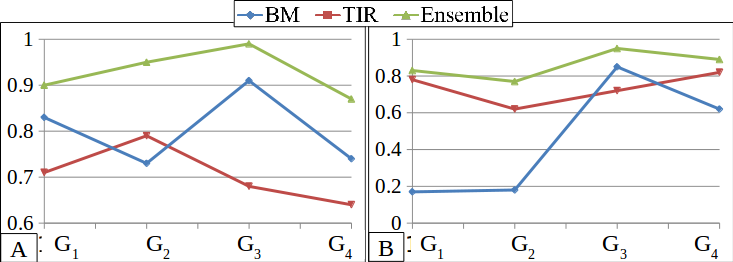
\includegraphics[width= 90mm]{Figures/Case1-2.png}
%\vspace{-10pt}
\caption{x-axis: global characteristics, y-axis: A)~Predictive accuracy for Case-1, B)~Predictive accuracy for Case-2}
%\vspace{-8pt}
\label{fig:case-1}
%\vspace{-8pt}
\end{figure}

Figure \ref{fig:case-1}, shows the prediction accuracy of four global characteristic for Case-1 and Case-2 respectively. Here, the accuracy is a ratio of correctly predicted products to the total number of products. In Case-1, accuracy of Ensemble model is in the range of 85 to 99\%  and it outperforms both SBM and UTS for all four global characteristics.

\textbf{\textit{Baseline Comparison}}: We also compared our approach with record matching method implemented in a framework called FEBRL\cite{christen2008febrl}. For attribute matching, we tried three similarity measures winkler, tokenset, trigam and show the results with winkler which outperforms the rest. We tested this approach for the Case-1 on the smaller dataset (5K products). Table~\ref{table:comparison}, shows the comparison of the prediction accuracy of four global attributes using our Ensemble approach and FEBRL. This suggests that our approach outperforms and also shows that accuracy of FEBRL decreases for high cardinality global attributes. FEBRL did not work on, 26k products, on a machine with 16GB RAM, Intel Core i7-3520M CPU 2.90GHz* 4, 64 bit. We did not try the blocking method as main motive of our problem is to improve accuracy of prediction, and not the time complexity. 
\renewcommand{\arraystretch}{}
\begin{table}
%\scriptsize 
  \centering
  %\small
  \begin{tabular}{|c|c|c|c|} 
   \hline
   Global att. & Num of states & FEBRL(winkler) & Ensemble \\
   \hline
   $G_1$ & 107 & 86\% & 93\% \\
   \hline
   $G_2$ & 154 & 57\% & 95.2\% \\
   \hline
   $G_3$ & 3 & 99.3\% & 99.2\% \\
   \hline
   $G_4$ & 13 & 95.4\% & 99.4\% \\
   \hline 
  \end{tabular}
  %\vspace{4pt}
\caption{Comparison of our approach with FEBRL}
  \label{table:comparison}
  %\vspace{-15pt}
\end{table}
\textbf{Case-2} (Figure \ref{fig:case-1}-B), naturally renders the SBM less accurate, since the training data contains only 10\% of possible states of each global characteristic. However, it is compensated by the performance of UTS, which searches the target set of global attribute values from the
retailer descriptions. Combining these models using our Ensemble model the accuracy of four global characteristics reaches 78 to 93\%.

\textbf{\textit{CoP Threshold for human annotation:}} We define three categories: a)~\textbf{P-C:} Number of products \textit{predicted correctly} by our approach for which CoP $> \tau$. b)~\textbf{P-I:} Number of products \textit{predicted incorrectly}, for which CoP $> \tau$. c)~ \textbf{NP:} Products which we choose \textit{not to predict}, i.e., products with CoP $\leq \tau$. We select $\tau$ in order to maximize P-C and minimize P-I category, while not increasing NP so much that exercise becomes almost entirely manual. Since products in the P-I category are more costly for a company as compared to NP category, we give more weight to P-I while learning $\tau$. Table~\ref{table:categories}, shows the percentage of products in each category (P-C, P-I, NP) on validation set along with the threshold $\tau$ values for both cases. It shows that for given $\tau$, percentage of products in P-C category is in the range of 81-96\% for Case-1, whereas, it ranges from 70 to 96\% for Case-2. Also, the average percentage of products in P-I category is only around 5\%. These numbers establish that CoP is a good measure for reliability of predictions. Figure~\ref{fig:PC-2}, shows the variation in the percentage of products in test set of each category with respect to threshold value $\tau$ for both Case-1 and Case-2, for the global characteristic $G_1$. It validates the optimal values of $\tau$ learned using validation set, 0.5 for Case-1 and 0.6 for Case-2.

The process of aggregate analysis, comparing global market share and sales of product categories is carried out in our platform \textbf{\textit{iFuse}}\cite{singh2016visual} (Figure~\ref{fig:iFuse}). Figure~\ref{fig:iFuse}(a),(b) shows the data tile and cart view of iFuse representing the attributes of the local DB and global DB to be linked together. Figure~\ref{fig:iFuse}(c) shows the tile view of the attributes obtained after mapping of local DB to global attribute, here GLO BRAND via ensemble approach, thereby enabling the \textbf{join} of local sales and global market share via common global attribute, GLO BRAND (Figure~\ref{fig:iFuse}(d)). Figure~\ref{fig:iFuse}(e) shows aggregate analysis of different products via motionchart.

\renewcommand{\arraystretch}{}
\begin{table}
  {%\scriptsize
  \centering
  \begin{tabular}{|p{0.7cm}|c|c|c|c|c|c|c|c|}
    \hline
    \multirow{2}{*}{Global} &
      \multicolumn{4}{c|}{Case-1} &
      \multicolumn{4}{c|}{Case-2} \\
      \cline{2-9}
    & $\tau$ & P-C & P-I & NP & $\tau$ & P-C & P-I & NP \\
   \hline
   $G_1$ & 0.5 & 92\% & 4\% & 4\% & 0.6 & 82\% & 7\% & 11\% \\
   \hline
   $G_2$ & 0.6 & 81\% & 7\% & 12\% & 0.65 & 74\% & 10\% & 16\% \\
   \hline
   $G_3$ & 0.7 & 96\% & 1\% & 3\% & 0.7 & 96\% & 1\% & 3\% \\
   \hline
   $G_4$ & 0.8 & 86\% & 3\% & 11\% & 0.8 & 85\% & 4\% & 11\% \\
   \hline
  \end{tabular}
  %\vspace{4pt}
  \scriptsize
  \caption{\% of products in each category on Validation set}
  \label{table:categories}
  %\vspace{-7pt}
  }
\end{table}

%\begin{figure}
%\centering
%\includegraphics[width = 65mm]{Figures/PC-PI-NP}
%\vspace{-8pt}
%\caption{Percentage of Products in each category for different values of $\tau$ on test data for $G_1$ in Case-1}
%\label{fig:PC-1}
%\vspace{-10pt}
%\end{figure}
%\vspace{-5pt}
\begin{figure}[!t]
\centering
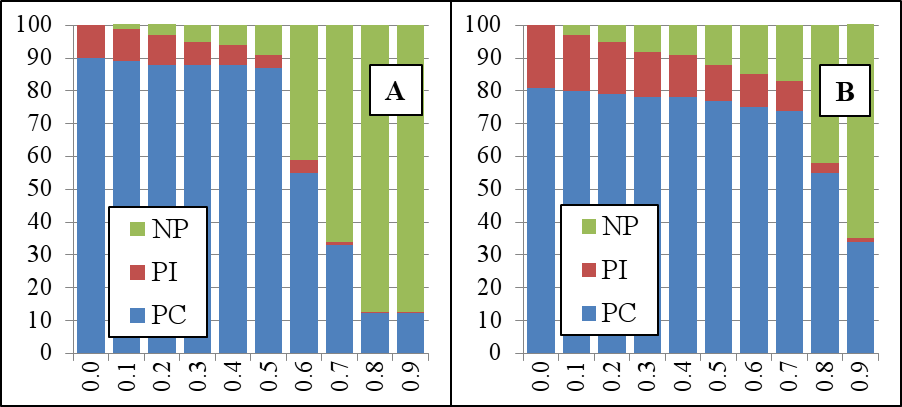
\includegraphics[width=100mm]{Figures/Fig67.png}
%\vspace{4pt}
\caption{\% of Products in each category for different values of $\tau$ on test data for $G_1$ in A)~Case-1 and	 B)~Case-2}
\label{fig:PC-2}
%\vspace{-14pt}
\end{figure}
\begin{figure}
\centering
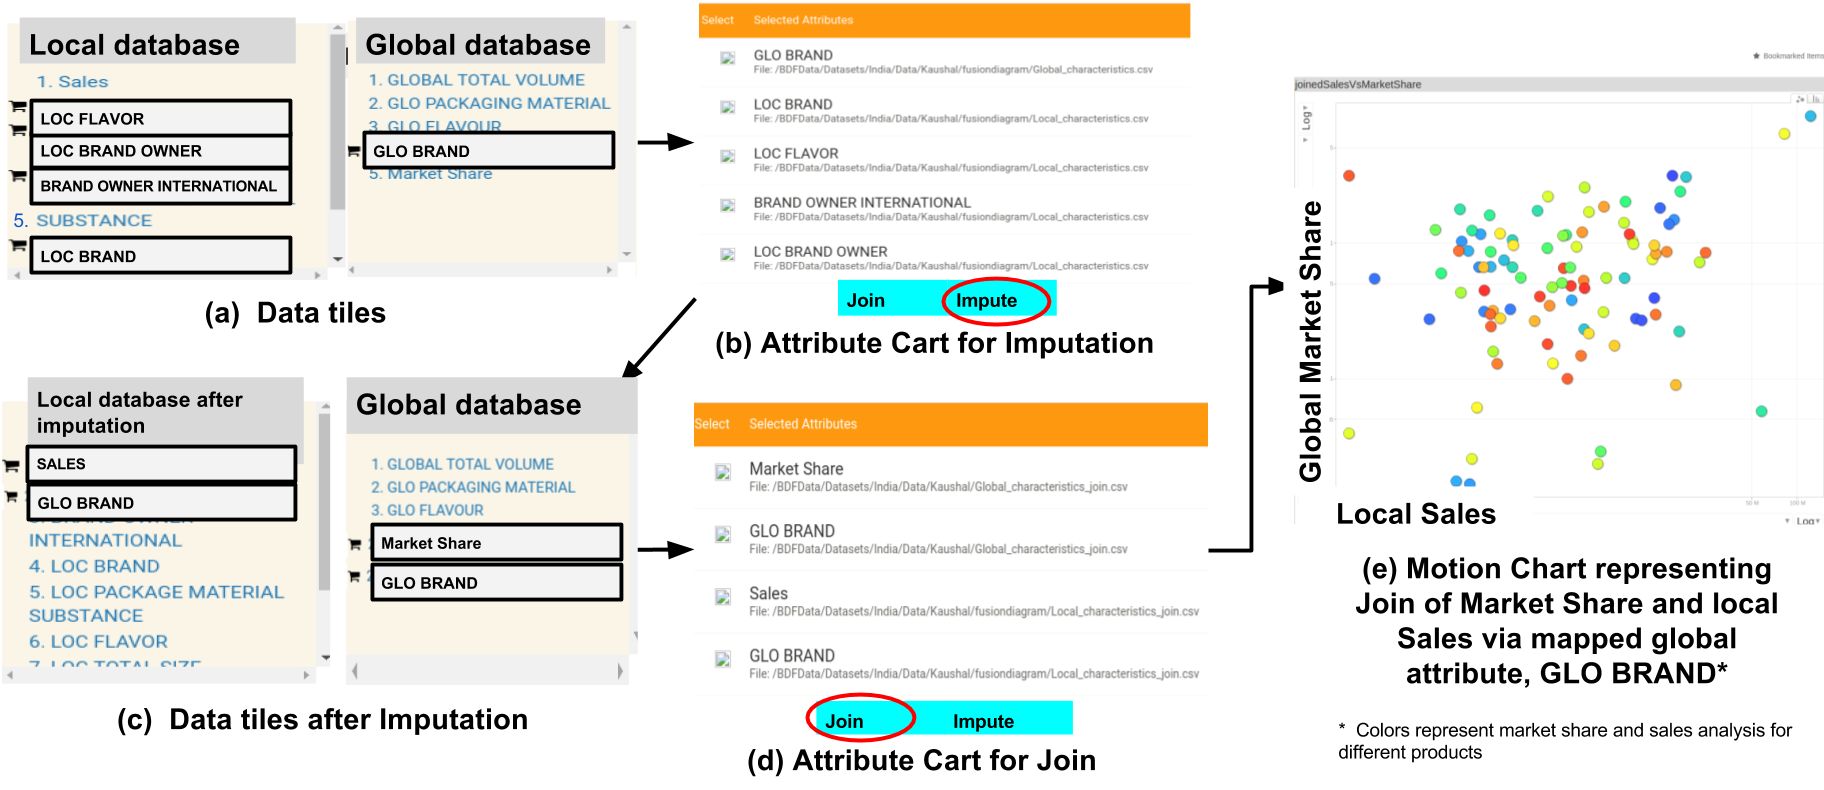
\includegraphics[width = 120mm]{Figures/EDBT_diagram3.png}
%\vspace{-8pt}
\caption{Figure showing aggregate analysis of global market share and local sales done using our platform. }
\label{fig:iFuse}
%\vspace{-12pt}
\end{figure}

% \begin{figure*}
% \centering
% \includegraphics[width=80mm]{Figures/iFuse}
% \vspace{1pt}
% \caption{jdd}
% \label{fig:iFuse}
% %\vspace{-16pt}
% \end{figure*}

\section{Conclusion}
\label{sec:conclusion}

This paper presents a matrix factorization based approach to text
outlier analysis. The approach is designed to adjust well to the
widely varying structures in different localities of the data, and
therefore provides more robust methods than competing models. The
approach has the potential to be applied to other domains with
similar structure, and as a specific example, we provide experiments
on market  basket data. We also presented extensive experimental
results, which illustrate the superiority of the approach.  
Our code can be downloaded from 
\url{https://github.com/ramkikannan/outliernmf} and 
tried with any text dataset. 

In this paper, we had a parallel implementation using the
Matlab's parallel computing toolbox to run in multicore environments.
In the future, we would like to explore a scalable implementation
of our algorithm. The solution is embarrassingly parallelizable,
and would like to experiment in web scale data. One of the potential
extension is incorporating temporal and spatial aspects into the model.
Such an extension, make the solution applicable to emerging 
applications such as topic detection and streaming data. 
%In the recent times,
%approximate matrix factorization techniques are explored by
%randomly sampling the input matrix. We can reduce the computation
%time for very large matrices using such sampling techniques. We would like
%to explore a sampling based solution for our model. 
We experimented
the solution primarily on text data and market basket data. In future
work, we will extend this broader approach to other domains such as
video data.


\subsubsection*{Acknowledgements}

This work was supported through funding from NSERC (Canada). We also thank Julien-Charles L\'evesque for insightful comments and Annette Schwerdtfeger for proofreading.

\bibliographystyle{plainnat}
%\bibliography{references,paper}
\bibliography{references}

\newpage
\appendix
{\LARGE\textbf{Appendix}}
%!TEX root = /Users/audrey/Dropbox/PhD/MOMAB/ArXiv/Latex/paper.tex

\section{Technical Tools}
\label{app:technical_tools}

\begin{fact}[$d$-dimensional Chernoff]
\label{fac:chernoffd}
    Let $X_1, \dots, X_N$ be i.i.d. $\sigma$-sub-Gaussian variables with values in such that $\Esp[X] = \mu$. Let $\hat \mu_N = \frac{1}{N} \sum_{i=1}^N X_i$. Then, as shown by \cite{Rigollet2015}, for any $a \geq 0$,
    \begin{align*}
        \Pr[|\hat \mu_N - \mu| \geq a] \leq 2 e^{-\frac{N a^2}{2 \sigma^2}}.
    \end{align*}
    Now consider the the multivariate setting where $\bsX_1, \dots, \bsX_N$ are i.i.d. $d$-dimensional $\sigma$-sub-Gaussian variables such that $\Esp[\bsX] = \bsmu$ and $\hat \bsmu_N = \frac{1}{N} \sum_{i=1}^N \bsX_i$. Then for any $a \geq 0$,
    \begin{align*}
        \Pr[\hat \bsmu_N \succeq \bsmu + a]
        & = \Pr[(\hat \mu_{N, 1} \geq \mu_1 + a) \wedge \dots \wedge (\hat \mu_{N, d} \geq \mu_d + a)]
        \leq e^{-\frac{d N a^2}{2 \sigma^2}}, \\
        \Pr[\hat \bsmu_N \not\preceq \bsmu + a]
        & \leq \Pr[(\hat \mu_{N, 1} \geq \mu_1 + a) \vee \dots \vee (\hat \mu_{N, d} \geq \mu_d + a)]
        \leq d e^{-\frac{N a^2}{2 \sigma^2}}, \\
        \Pr[\hat \bsmu_N \not\in B(\bsmu, a)]
        & \leq \Pr[(|\hat \mu_{N, 1} - \mu_1| \geq a) \vee \dots \vee (|\hat \mu_{N, d} - \mu_d| \geq a)]
        \leq 2 d e^{-\frac{N a^2}{2 \sigma^2}}.
    \end{align*}
\end{fact}

\begin{fact}[$d$-dimensional Gaussian concentration]
\label{fac:concentration}
    Let $X$ be a Gaussian random variable with mean $\mu$ and standard deviation $\sigma$. The following concentration is derived~\cite{Agrawal2013} from \cite{Abramowitz1964} for $z \geq 1$:
    \begin{align*}
        \Pr[|X - \mu| > z \sigma] \leq \frac{1}{2} e^{-z^2/2}.
    \end{align*}
    Now consider the multivariate setting where $\bsX$ denotes a $d$-dimensional Gaussian random variable with mean $\bsmu$ and diagonal covariance $\bsSigma$. Then for $z \geq 1$,
    \begin{align*}
        \Pr[\bsX \succ \bsmu + z \sqrt{\diag(\bsSigma)}]
        & = \Pr[(X_1 > \mu_1 + z \sigma_1) \wedge \dots \wedge (X_d > \mu_d + z \sigma_d)]
        \leq \bigg( \frac{1}{4} e^{-z^2/2} \bigg)^d, \\
        \Pr[\bsX \not\prec \bsmu + z \sqrt{\diag(\bsSigma)}]
        & \leq \Pr[(X_1 \geq \mu_1 + z \sigma_1) \vee \dots \vee (X_d \geq \mu_d + z \sigma_d)]
        \leq \frac{d}{4} e^{-z^2/2}, \\
        \Pr[\bsX \not\in B(\bsmu, z \sqrt{\diag(\bsSigma)})]
        & \leq \Pr[(|X_1 - \mu_1| \geq z \sigma_1) \vee \dots \vee (|X_d - \mu_d| \geq z \sigma_d)]
        \leq \frac{d}{2} e^{-z^2/2}.
    \end{align*}
\end{fact}

\begin{fact}[$d$-dimensional Gaussian anti-concentration]
\label{fac:anti_concentration}
    Let $X$ be a Gaussian random variable with mean $\mu$ and standard deviation $\sigma$. The following concentration is derived~\cite{Agrawal2013} from \cite{Abramowitz1964} for $z \geq 1$:
    \begin{align*}
        \Pr[X > \mu + z \sigma] \geq \frac{z}{\sqrt{2 \pi} (z^2 + 1)} e^{-z^2/2}.
    \end{align*}
    Now consider the multivariate setting where $\bsX$ denotes a $d$-dimensional Gaussian random variable with mean $\bsmu$ and diagonal covariance $\bsSigma$. Then for $z \geq 1$,
    \begin{align*}
        \Pr[\bsX \succ \bsmu + z \sqrt{\diag(\bsSigma)}]
        & = \Pr[(X_1 > \mu_1 + z \sigma_1) \wedge \dots \wedge (X_d > \mu_d + z \sigma_d)]
        \geq \bigg( \frac{z}{\sqrt{2 \pi} (z^2 + 1)} e^{-z^2/2} \bigg)^d.
    \end{align*}
\end{fact}


\section{Proof of Lemma~\ref{lem:counts_before_succ}}
\label{app:proof:counts_before_succ}

\begin{proof}
    Let $\Theta_j$ denote a $\Normal_d (\hat \bsmu_\star(\tau_j+1), (I_d + N_\star(\tau_j+1)I_d)^{-1})$ distributed multivariate normal random variable. Let $G_j$ be a geometric variable denoting the number of consecutive independent trials until $\Theta_j \succ \bsmu_\star - \rho_\star$. Then observe that 
    \begin{align*}
         \Esp \bigg[ \sum_{t=\tau_k+1}^{\tau_{k+1}} \Pr[\bstheta_\star(t) \not\succ \bsmu_\star - \rho_\star | \cF_t] \bigg]
         \leq \Esp[G_j]
         = \sum_{i = 1}^\infty \Pr[G_j \geq i].
    \end{align*}
    We want to bound the expected value of $G_j$ by a constant for all $j$. Consider any integer $i \geq 1$, let $z = \sqrt{\ln i^{1/d}}$, and let $\mathrm{MAX}_i$ denote the \emph{maximum preference} of $i$ independent samples of $\Theta_j$, that is $\max_{1 \leq i \leq j} f(\Theta_j)$. We abbreviate $\hat \bsmu_\star(\tau_j+1)$ as $\hat \bsmu_\star$ and $N_\star(\tau_j+1)$ as $N_\star$ in the following. Then
    \begin{align*}
        \Pr[G_j < i]
        & \geq \Pr[\mathrm{MAX}_i \succ \bsmu_\star - \rho_\star] \\
        & \geq \Pr \Big[ \mathrm{MAX}_i \succ \hat \bsmu_\star + \frac{z}{\sqrt{N_\star}} \Big| \hat \bsmu_\star + \frac{z}{\sqrt{N_\star}} \succeq \bsmu_\star - \rho_\star \Big]
        \cdot \Pr \Big[ \hat \bsmu_\star + \frac{z}{\sqrt{N_\star}} \succeq \bsmu_\star - \rho_\star \Big].
    \end{align*}
    Using Fact~\ref{fac:anti_concentration}, this gives
    \begin{align*}
        \Pr \Big[ \mathrm{MAX}_i \succ \hat \bsmu_\star + \frac{z}{\sqrt{N_\star}} \Big| \hat \bsmu_\star + \frac{z}{\sqrt{N_\star}} \succeq \bsmu_\star - \rho_\star \Big]
        & \geq 1 - \Bigg( 1 - \bigg( \frac{1}{\sqrt{2\pi}} \frac{z}{z^2 + 1} e^{-z^2/2} \bigg)^d \Bigg)^i \\
        & = 1 - \Bigg( 1 - \bigg( \frac{1}{\sqrt{2\pi}} \frac{\sqrt{\ln i^{1/d}}}{(\ln i^{1/d} + 1)} \frac{1}{\sqrt{i^{1/d}}} \bigg)^d \Bigg)^i \\
        & \geq 1 - \Bigg( 1 - \bigg( \frac{1}{\sqrt{18 \pi d i^{1/d} \ln i}} \bigg)^d \Bigg)^i \\
        & \geq 1 - e^{-\frac{\sqrt{i}}{\sqrt{18 \pi d \ln i}^d}},
    \end{align*}
    where the second inequality uses that $\ln i^{1/d} + 1 < 3 \ln i$ and the last inequality uses that $1 - x < e^{-x}$. Also, using Fact~\ref{fac:chernoffd}, we have
    \begin{align*}
        \Pr[\hat \bsmu_\star \succeq \bsmu_\star - \frac{z}{\sqrt{N_\star}}]
        \geq 1 - d e^{-\frac{z^2}{2\sigma^2}}
        = 1 - \frac{d}{i^{1/(2d\sigma^2)}}.
    \end{align*}
    Substituting, we obtain
    \begin{align*}
        \Pr[G_j < i]
        \geq \Big( 1 - e^{-\frac{\sqrt{i}}{\sqrt{4 \pi \ln i}^d}} \Big) \cdot \Big( 1 - \frac{d}{i^{1/(2d\sigma^2)}} \Big)
        \geq 1 - \frac{d}{i^{1/(2d\sigma^2)}} - e^{-\frac{\sqrt{i}}{\sqrt{18 \pi d \ln i}^d}}
    \end{align*}
    and
    \begin{align*}
        \Esp[G_j]
        & = \sum_{i \geq 1} (1 - \Pr[G_j < i]) \\
        & \leq \sum_{i \geq 1} \Big( \frac{d}{i^{1/(2d\sigma^2)}} + e^{-\frac{\sqrt{i}}{\sqrt{18 \pi d \ln i}^d}} \Big) \\
        & \leq C(d) + 2 d \sum_{i \geq 1} \frac{1}{i^{1/(2d\sigma^2)}},
    \end{align*}
    where $C(d)$ is such that $e^{-\frac{\sqrt{i}}{\sqrt{18 \pi d \ln i}^d}} \leq \frac{d}{i^{1/(2d\sigma^2)}}$ for $i \geq C(d)$. We observe that $\sigma^2 \leq 1/(4d)$ is required in order for the sum to converge.
\end{proof}



\end{document}
